\begin{figure} [h]
    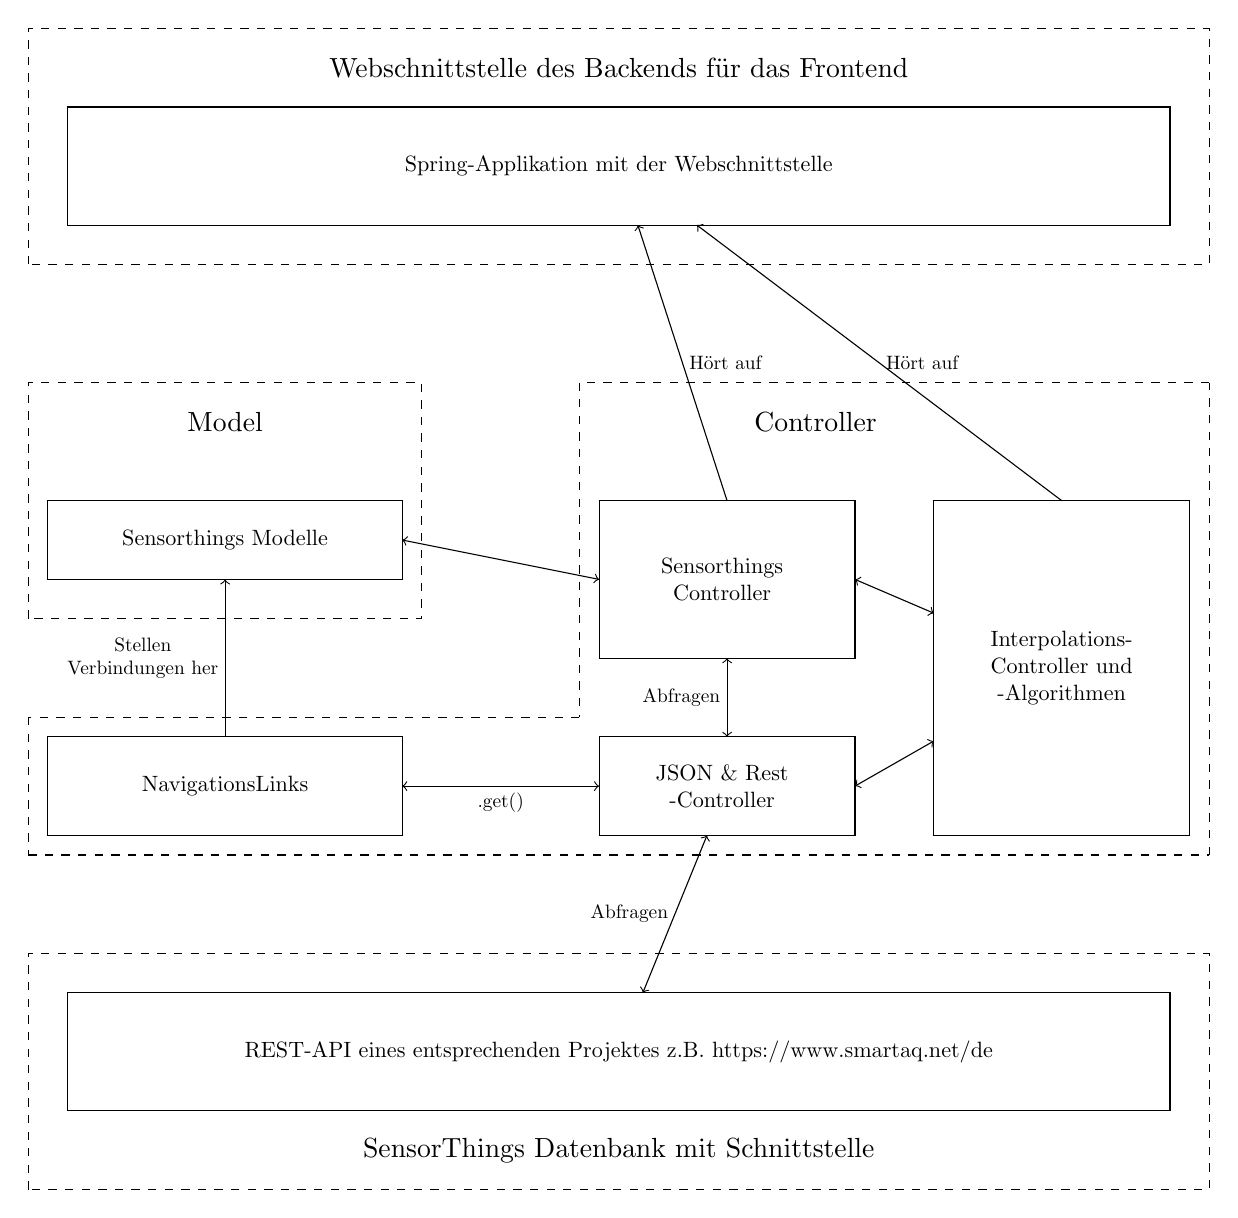
\begin{tikzpicture}[node distance=2cm]

        %SPRING
        \begin{scope}[shift={(0,11.75)},local bounding box=SPRING]
            \draw (0,0) [dashed] rectangle (15,3);
            \node[scale=1] at (7.5,2.5) {Webschnittstelle des Backends für das Frontend};
            \begin{scope}[local bounding box=SPRINGWEB]
                \draw (0.5,0.5) rectangle (14.5,2);
                \node[scale=0.8, align=center] at (7.5,1.25) {Spring-Applikation mit der Webschnittstelle};
            \end{scope}
        \end{scope}

        %Model
        \begin{scope}[shift={(0,4.25)},local bounding box=SensorThings]
            \draw (0,3) [dashed] rectangle (5,6);
            \node[scale=1] at (2.5,5.5) {Model};
            \begin{scope}[local bounding box=SensorthingsM]
                \draw (0.25,3.5) rectangle (4.75,4.5);
                \node[scale=0.8] at (2.5,4) {Sensorthings Modelle};
            \end{scope}
            \begin{scope}[local bounding box=Link]
                \draw (0.25,0.25) rectangle (4.75,1.5);
                \node[scale=0.8] at (2.5,.875) {NavigationsLinks};
            \end{scope}
        \end{scope}
        
        %Controller
        \begin{scope}[shift={(7,4.25)},local bounding box=Backend]
            %\draw (0,0) [dashed] rectangle (8,6);
            \draw [dashed] (-7,0) -- (8,0);
            \draw [dashed] (8,0) -- (8,6);
            \draw [dashed] (8,6) -- (0,6);
            \draw [dashed] (0,6) -- (0,1.75);
            \draw [dashed] (0,1.75) -- (-7,1.75);
            \draw [dashed] (-7,1.75) -- (-7,0);
            \node[scale=1] at (3,5.5) {Controller};
            \begin{scope}[local bounding box=STController]
                \draw (0.25,2.5) rectangle (3.5,4.5);
                \node[scale=0.8,align=center] at (1.8125,3.5) {Sensorthings\\Controller};
            \end{scope}
            \begin{scope}[local bounding box=JSONREST]
                \draw (0.25,0.25) rectangle (3.5,1.5);
                \node[scale=0.8, align=center] at (1.8125,.875) {JSON \& Rest\\-Controller};
            \end{scope}
            \begin{scope}[local bounding box=Interpolation]
                \draw (4.5,0.25) rectangle (7.75,4.5);
                \node[scale=0.8, align=center] at (6.125,2.375) {Interpolations-\\Controller und\\-Algorithmen};
            \end{scope}
        \end{scope}

        %Sensorthings Datenbank
        \begin{scope}[shift={(0,0)},local bounding box=Backend]
            \draw (0,0) [dashed] rectangle (15,3);
            \node[scale=1] at (7.5,0.5) {SensorThings Datenbank mit Schnittstelle};
            \begin{scope}[local bounding box=SensorthingsAPI]
                \draw (0.5,1) rectangle (14.5,2.5);
                \node[scale=0.8, align=center] at (7.5,1.75) {REST-API eines entsprechenden Projektes z.B. https://www.smartaq.net/de};
            \end{scope}
        \end{scope}

        \draw[->] (Link.north) -- (SensorthingsM.south) node[midway,left,scale=0.7,align=center] {Stellen\\Verbindungen her};
        \draw[<->] (SensorthingsAPI) -- (JSONREST) node[midway,left,scale=0.7,align=center] {Abfragen};
        \draw[<->] (Link.east) -- (JSONREST.west) node[midway,below,scale=0.7,align=center] {.get()};
        \draw[<->] (JSONREST.north) -- (STController.south) node[midway,left,scale=0.7,align=center] {Abfragen};
        \draw[<->] (SensorthingsM.east) -- (STController.west);
        \draw[<->] (Interpolation) -- (STController.east);
        \draw[<->] (Interpolation) -- (JSONREST.east);
        \draw[<-] (SPRINGWEB) -- (Interpolation.north) node[midway,right,scale=0.7,align=center] {Hört auf};
        \draw[<-] (SPRINGWEB) -- (STController.north) node[midway,right,scale=0.7,align=center] {Hört auf};
    \end{tikzpicture}
    \caption{Aufbau des \softwarename Backends}
\end{figure}